\section{Second-order correlation analysis}

In this section, we analyse the effectiveness of the implemented countermeasures against second-order side-channel analysis based on the linear correlation coefficient (CPA). For this study, we will target the Sbox output value and consider a Hamming weight ($HW$) univariate leakage model.

In the remainder of this section, we will use:
\begin{itemize}

\item the centered product combination function $\mathcal{C}(x,y) = (x-\bar{x})(y-\bar{y})$ to preprocess the traces, where $\bar{x}$ (resp. $\bar{y}$) stands for the mean value of $x$ (resp. $y$), computed on all traces in our campaign; 

\item the corresponding function $f_{HW}(z) = \sum_m (HW(z \oplus m) - \overline{HW(z\oplus m)})\\(HW(m)-\overline{HW(m)})$ to compute the predictions, where $\overline{HW(m)}$ (resp $\overline{HW(z \oplus m)}$) stands for the mean value of $HW(m)$ (resp. $HW(z\oplus m)$) computed on all possible values of $m$\footnote{Note that all possible values for $m$ are in $[0,255]$.}.
\end{itemize}

As in our first-order correlation analysis, we will split this study in two parts. The first part will consider priviledged knowledge on the mask values. The second part will not take this knowledge into account.

\subsection{Priviledged knowledge}
We first study the setting where the attacker knows the random masks used to compute the permutation. 
In order to characterize the effectiveness of a CPA against this implementation, we use the random masks to recompute the permutation $Sh(i)$ for each byte index $i$.

For each byte index $i$, we use the characterization phase to isolate a window $w_{z\oplus m}$ of $11$ points of interest corresponding to the manipulation of the Sbox output $\rmult \times S[P[Sh(i)\oplus K[Sh(i)]] \oplus \rout$, and a window $w_m$ of $11$ points of interest corresponding to the manipulation of the mask value $\rout$. For each couple $(i,j)$ of points in $w_{z\oplus m} \times w_m$, we apply the combination function $\mathcal{C}(i,j)$.

\noindent We then perform an attack targeting the value $Z_{\hat{k}}[i]=S[P[Sh(i)] \oplus K[Sh(i)] \oplus \hat{k}]$, where $\hat{k}$ is an hypothesis on a value of one byte.


\subsubsection{Multiplicatively masked Sbox output}
We suppose the knowledge of the multiplicative mask $\rmult$. This knowledge allows for the prediction of the value $\rmult \times Z_{\hat{k}}[i]$ for any hypothesis $\hat{k}$.
The attack succeeds with around $8.000$ traces to $20.000$ traces.
Figure~\ref{fig:CPA2O_trickedaZ1} illustrates the results using $20.000$ traces.

\begin{figure}[H]
	\centering 
	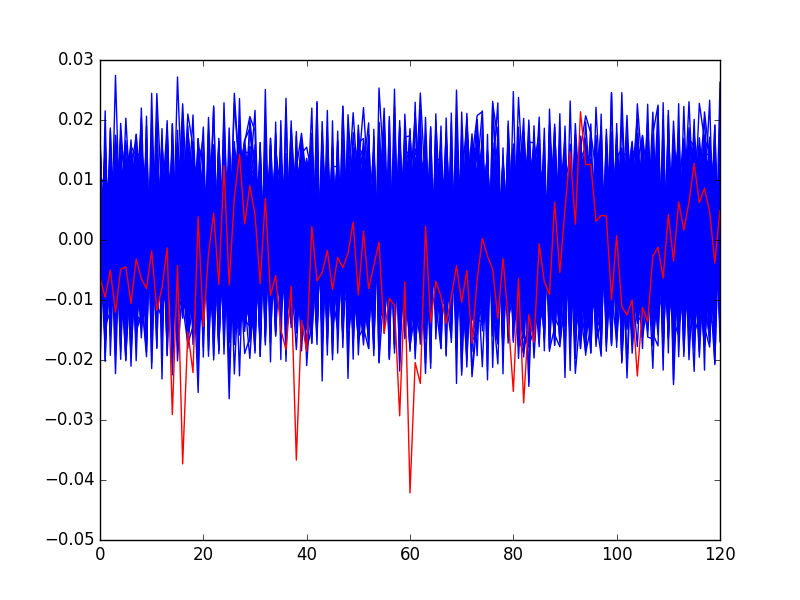
\includegraphics[scale=0.35]{figures/CPA2O_trickedaZ1.png}
	\caption{Correlation coefficients obtained when targeting $\rmult \times S[P[i]\oplus \hat{k}] $, for every value of $\hat{k}$. Correct hypothesis plotted in red. X-axis represents all 121 points combinations.}
	\label{fig:CPA2O_trickedaZ1}
\end{figure}


\subsubsection{Raw Sbox output}
We target the value $Z_{\hat{k}}[i]$ for any hypothesis $k$.
The attack does not succeed using the $100.000$ traces.
Figure~\ref{fig:CPA2O_trickedZ1} illustrates the results using $100.000$ traces.

\begin{figure}[H]
	\centering 
	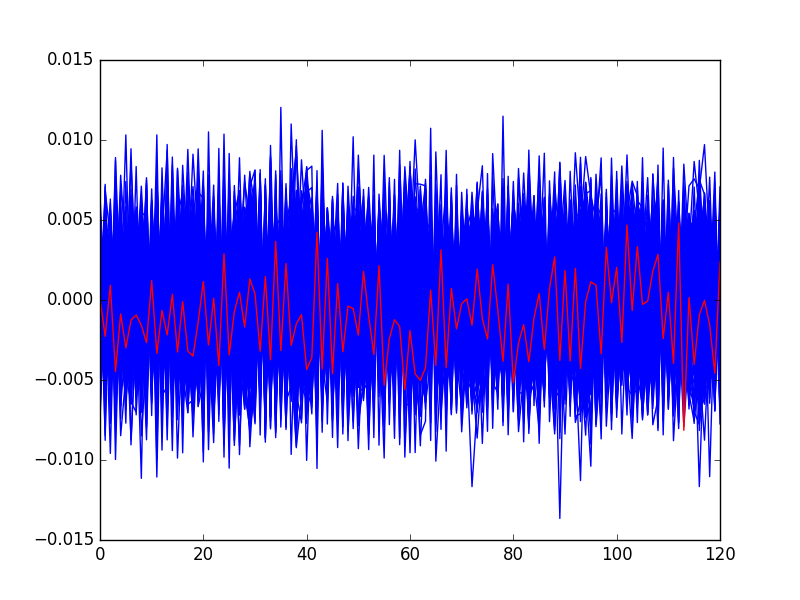
\includegraphics[scale=0.35]{figures/CPA2O_trickedZ1.png}
	\caption{Correlation coefficients obtained when targeting $S[P[i]\oplus \hat{k}] $, for every value of $\hat{k}$. Correct hypothesis plotted in red. X-axis represents all 121 points combinations.}
	\label{fig:CPA2O_trickedZ1}
\end{figure}


\subsection{Unknown permutation, processed traces}
We now study the setting where the attacker does not know the random masks used to compute the permutation.
We preprocess the traces in order to average the leakage over the different byte indices manipulation:
\begin{itemize}
	\item for each index $i$ in $[0,15]$, we define a small window $w_i$ of $\ell$ points around the SNR peak corresponding to the manipulation of $\rmult \times S[P[Sh(i)] \oplus K[Sh(i)]]\oplus \rout$ in the characterization phase. In our experiments, the size of the window was arbitrarily fixed to $\ell=11$.
	\item for each trace in our acquisition campaign, we compute the average window $m$ such that for each time sample $j$, $m[j]=\frac{1}{16}\sum_{i=0}^{15} w_i[j]$. We then consider $m$ as our reduced averaged trace of size $\ell$.
	\item we concatenate to this trace a small window of $\ell$ points around the SNR peak corresponding to the manipulation of $\rout$.
\end{itemize}

\subsubsection{Multiplicatively masked Sbox output}
We suppose the knowledge of the multiplicative mask $\rmult$. This knowledge allows for the prediction of the value $\rmult \times Z_{\hat{k}}[i]$ for any hypothesis $\hat{k}$.
The attack is unsuccessful using $100.000$ traces.

Figure~\ref{fig:CPA2O_averagedaZ1} illustrates the results using $100.000$ traces.
\begin{figure}[H]
	\centering 
	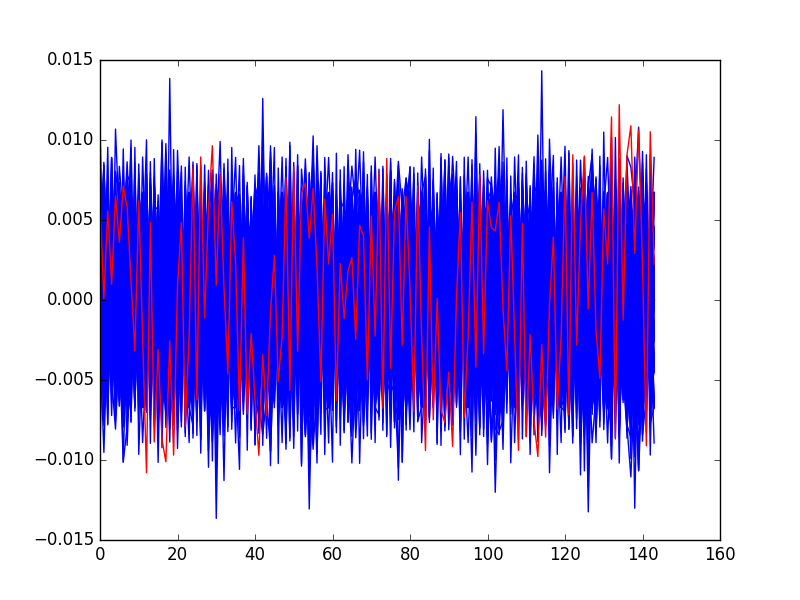
\includegraphics[scale=0.35]{figures/CPA2O_averagedaZ1.png}
	\caption{Correlation coefficients obtained when targeting $\rmult \times S[P[i]\oplus \hat{k}] $, for every value of $\hat{k}$. Correct hypothesis plotted in red. X-axis represents all 121 points combinations.}
	\label{fig:CPA2O_averagedaZ1}
\end{figure}

However, we observe that, for certain combinations of points (around abscissa 135), the correct hypothesis is indeed the most likely. Furthermore, the rank convergence of the key, plotted on Figure~\ref{fig:convergence}, might indicate that the attack could be successful when using more traces.

\begin{figure}[H]
	\centering 
	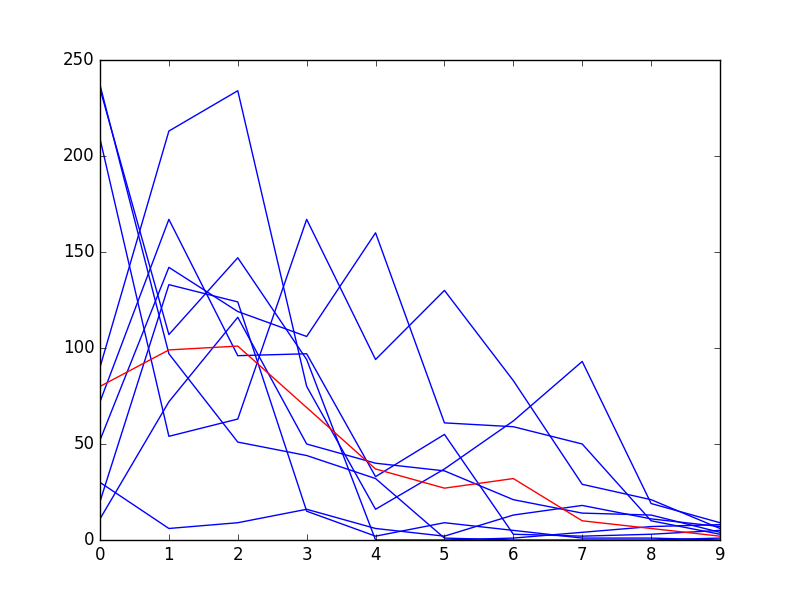
\includegraphics[scale=0.35]{figures/convergence.png}
	\caption{Rank of the ten best-ranked keys, by steps of 10000 measurements, from $10.000$ to $100.000$. Correct key plotted in red.}
	\label{fig:convergence}
\end{figure}

\subsubsection{Raw Sbox output}
We target the value $Z_{\hat{k}}[i]$ for any hypothesis $\hat{k}$.
The attack does not succeed using the $100.000$ traces.
Figure~\ref{fig:CPA2O_averagedZ1} illustrates the results using $100.000$ traces.
\begin{figure}[H]
	\centering 
	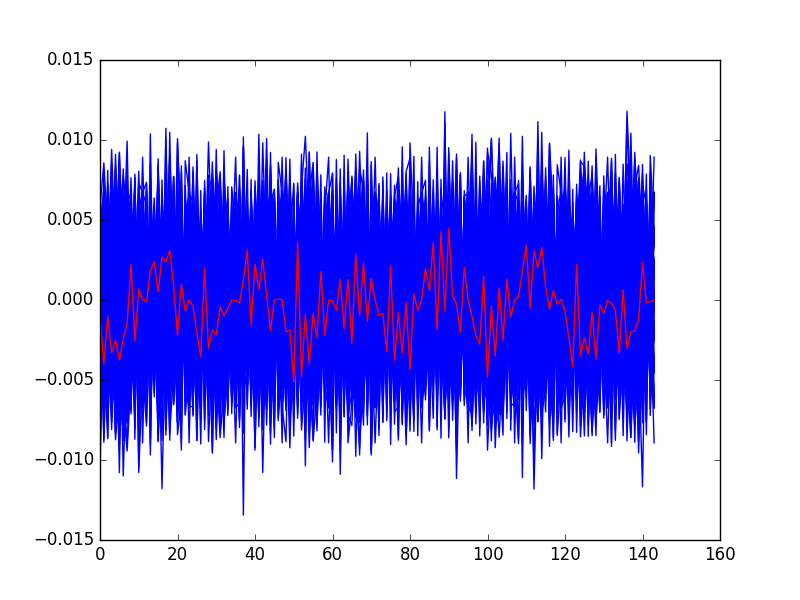
\includegraphics[scale=0.35]{figures/CPA2O_averagedZ1.png}
	\caption{Correlation coefficients obtained when targeting $S[P[i]\oplus \hat{k}] $, for every value of $\hat{k}$. Correct hypothesis plotted in red. X-axis represents all 121 points combinations.}
	\label{fig:CPA2O_averagedZ1}
\end{figure}


\subsection{Unknown permutation, non-processed traces}
For the sake of completeness, we also perform these experiments on raw unprocessed traces. No success is obtained when targeting $Z_{\hat{k}}[i]$ or $\rmult \times Z_{\hat{k}}[i]$.

No attack is successful using $100.000$ traces.

\subsection{Summary}
This section evidences the effectiveness of the implemented countermeasures. 
The shuffling countermeasures increases the number of needed measurements by a factor of at least $\frac{100.000}{8.000} = 12,5$. It is however likely that this countermeasure does not suffice when increasing slightly the number of measurements.
The effectiveness of the affine countermeasure is evidenced by the fact that a 2OCPA is achievable targeting the value $\rmult \times S[P[i] \oplus \hat{k}]$
but no attack is found targeting the value $S[P[i] \oplus \hat{k}]$ using $100.000$ traces.

\begin{figure}[h!]
\centering
\begin{tabular}{|c|c|c|c|c|}
  \hline
   & \multicolumn{2}{c|}{Known permutation}&\multicolumn{2}{c|}{Unknown permutation}\\
  \hline
  Known & $\rmult $ &  None  & $\rmult $  &  None \\
  \hline
  \# Traces& $\approx 8.000$ & $ > 100.000$ & $ > 100.000$ & $> 100.000$\\
  \hline
\end{tabular}
\caption{Number of traces needed for a successful second-order attack, in the different settings.}
\end{figure}


